\chapter{class Lfsr}

\index{LFSR}
\Lfsr\ is an object type allowing to simulate and analyze any type of Linear Feedback Shift Register. Simulations are performed using \texttt{bitarray} objects, where \texttt{bitarray\_object[N]} holds value of Flip-Flop having index \textit{N}. \Lfsr\ objects are always simulated assuming, that data is shifted from higher to lower indexed flip-flop (from FF[1] to FF[0], from FF[2] to FF[1] and so on).

\section{Lfsr types}

\subsection{Fibonacci}

\index{LFSR!Fibonacci}
\index{Fibonacci LFSR}

Look at the Figure \ref{lfsr:fibonacci}. It shows an example of Fibonacci LFSR implementing the polynomial of $x^8+x^6+x^5+x^2+1$. There are couple of ways to create such \Lfsr\ object:

\begin{lstlisting}[language=Python]
	# using existing Polynomial object:
	p1 = Polynomial([8,6,5,2,0])
	lfsr1 = Lfsr(p1, FIBONACCI)
	# using Polynomial created in place:
	lfsr1 = Lfsr(Polynomial([8,6,5,2,0]), FIBONACCI)
	# using coefficients list:
	lfsr1 = Lfsr([8,6,5,2,0], FIBONACCI)
\end{lstlisting}

\begin{figure}[h]
	\centering
	\scalebox{.75}{\newcommand{\drawff}[2]{		
	\fill[black!5!white] 		($#1-(0.5, 0.5)$)	rectangle	($#1+(0.5, 0.5)$);
	\draw[thick] 		($#1-(0.5, 0.5)$)	rectangle	($#1+(0.5, 0.5)$);
	\node[] at ($#1+(0.0, 0.0)$) {\large#2};
}
\newcommand{\drawfibonacciconnector}[2]{
	\draw[-latex] ($#1+(0.0, 0.0)$) -- ($#1+(0.0, 2.0)-(0.0,0.25)$);
	\fill[black]  ($#1+(0.0, 0.0)$) circle (0.07);
	\fill[black!5!white]  ($#1+(0.0, 2.0)$) circle (0.25);
	\draw[thick]  ($#1+(0.0, 2.0)$) circle (0.25);
	\draw[thick]  ($#1+(0.0, 2.0)-(0.25,0.0)$) -- ($#1+(0.0, 2.0)+(0.25,0.0)$);
	\draw[thick]  ($#1+(0.0, 2.0)-(0.0,0.25)$) -- ($#1+(0.0, 2.0)+(0.0,0.25)$);
	\draw[latex-] ($#1+(0.0, 2.0)+(0.25,0.0)$) -- ($#1+(0.0, 2.0)+(0.5,0.0)$);
	\node[anchor=west] at ($#1+(0.0, 1.2)$) {\Large#2};
}
\begin{tikzpicture}
	\draw (-1,0) rectangle (15,2);
	\drawff {(0,0)} {7}
	\drawff {(2,0)} {6}
	\drawfibonacciconnector {(3,0)} {$x^6$}
	\drawff {(4,0)} {5}
	\drawfibonacciconnector {(5,0)} {$x^5$}
	\drawff {(6,0)} {4}
	\drawff {(8,0)} {3}
	\drawff {(10,0)} {2}
	\drawfibonacciconnector {(11,0)} {$x^2$}
	\drawff {(12,0)} {1}
	\drawff {(14,0)} {0}
	\draw[-latex] (-1.0,0.0) -- (-0.5,0.0);
\end{tikzpicture}}
	\caption{Fibonacci LFSR implementing polynomial $x^8+x^6+x^5+x^2+1$.}
	\label{lfsr:fibonacci}
\end{figure}

\subsection{Galois}

\index{LFSR!Galois}
\index{Galois LFSR}

Figure \ref{lfsr:fibonacci} shows an example of Galois LFSR implementing the polynomial of $x^8+x^6+x^5+x^2+1$. There are couple of ways to create such \Lfsr\ object:

\begin{lstlisting}[language=Python]
	# using existing Polynomial object:
	p1 = Polynomial([8,6,5,2,0])
	lfsr1 = Lfsr(p1, GALOIS)
	# using Polynomial created in place:
	lfsr1 = Lfsr(Polynomial([8,6,5,2,0]), GALOIS)
	# using coefficients list:
	lfsr1 = Lfsr([8,6,5,2,0], GALOIS)
\end{lstlisting}

\begin{figure}[h]
	\centering
	\scalebox{.75}{\newcommand{\drawff}[2]{		
	\fill[black!5!white] 		($#1-(0.5, 0.5)$)	rectangle	($#1+(0.5, 0.5)$);
	\draw[thick] 		($#1-(0.5, 0.5)$)	rectangle	($#1+(0.5, 0.5)$);
	\node[] at ($#1+(0.0, 0.0)$) {\large#2};
}
\newcommand{\drawgaloisconnector}[2]{
	\draw[latex-] ($#1+(0.0, 0.25)$) -- ($#1+(0.0, 2.0)-(0.0,0.0)$);
	\fill[black]  ($#1+(0.0, 2.0)$) circle (0.07);
	\fill[black!5!white]  ($#1+(0.0, 0.0)$) circle (0.20);
	\draw[thick]  ($#1+(0.0, 0.0)$) circle (0.2);
	\draw[thick]  ($#1+(0.0, 0.0)-(0.2,0.0)$) -- ($#1+(0.0, 0.0)+(0.2,0.0)$);
	\draw[thick]  ($#1+(0.0, 0.0)-(0.0,0.2)$) -- ($#1+(0.0, 0.0)+(0.0,0.2)$);
	\draw[latex-] ($#1+(0.0, 0.0)-(0.5,0.0)$) -- ($#1+(0.0, 0.0)-(0.2,0.0)$);
	\node[anchor=west] at ($#1+(0.0, 1.2)$) {\Large#2};
}
\begin{tikzpicture}
	\draw (-1,0) rectangle (15,2);
	\drawff {(0,0)} {7}
	\drawff {(2,0)} {6}
	\drawgaloisconnector {(3,0)} {$x^6$}
	\drawff {(4,0)} {5}
	\drawgaloisconnector {(5,0)} {$x^5$}
	\drawff {(6,0)} {4}
	\drawff {(8,0)} {3}
	\drawff {(10,0)} {2}
	\drawgaloisconnector {(11,0)} {$x^2$}
	\drawff {(12,0)} {1}
	\drawff {(14,0)} {0}
	\draw[-latex] (-1.0,0.0) -- (-0.5,0.0);
\end{tikzpicture}}
	\caption{Galois LFSR implementing polynomial $x^8+x^6+x^5+x^2+1$.}
	\label{lfsr:galois}
\end{figure}

\subsection{Ring Generator}

\index{LFSR!Ring Generator}
\index{Ring Generator}

Ring generator is a structure discussed in \cite{lfsr:fastsim}. Example of a Ring Generator is shown in the Figure \ref{lfsr:ring} implementing the polynomial $x^8+x^6+x^5+x^2+1$. Ways to create such object are:

\begin{lstlisting}[language=Python]
	# using existing Polynomial object:
	p1 = Polynomial([8,6,5,2,0])
	lfsr1 = Lfsr(p1, RING_GENERATOR)
	# using Polynomial created in place:
	lfsr1 = Lfsr(Polynomial([8,6,5,2,0]), RING_GENERATOR)
	# using coefficients list:
	lfsr1 = Lfsr([8,6,5,2,0], RING_GENERATOR)
\end{lstlisting}

\begin{figure}[h]
	\centering
	\scalebox{.75}{\newcommand{\drawff}[2]{		
	\fill[black!5!white] 		($#1-(0.5, 0.5)$)	rectangle	($#1+(0.5, 0.5)$);
	\draw[thick] 		($#1-(0.5, 0.5)$)	rectangle	($#1+(0.5, 0.5)$);
	\node[] at ($#1+(0.0, 0.0)$) {\large#2};
}
\newcommand{\drawring}[2]{
	\coordinate (A) at ($#1-(1.0,0.0)$);
	\coordinate (A2) at ($(A)+(0.5,0.0)$);
	\coordinate (B) at ($#2+(1.0,0.0)$);
	\coordinate (B2) at ($(B)-(0.5,0.0)$);
	\draw (A) rectangle (B);
	\draw[-latex] (A) -- (A2);
	\draw[-latex] (B) -- (B2);
}
\newcommand{\drawringconnectorup}[3]{
	\coordinate (A) at ($#1+(0.0,1.0)$);
	\coordinate (B) at ($#2-(0.0,1)$);
	\coordinate (C) at ($0.3*(B)+0.7*(A)+(0.0,0.2)$);
	\draw[-latex] #1 -- (A) -- (B) -- ($#2-(0.0,0.2)$);
	\fill[black]  ($#1+(0.0, 0.0)$) circle (0.07);
	\fill[black!5!white]  ($#2+(0.0, 0.0)$) circle (0.20);
	\draw[thick]  ($#2+(0.0, 0.0)$) circle (0.2);
	\draw[thick]  ($#2+(0.0, 0.0)-(0.2,0.0)$) -- ($#2+(0.0, 0.0)+(0.2,0.0)$);
	\draw[thick]  ($#2+(0.0, 0.0)-(0.0,0.2)$) -- ($#2+(0.0, 0.0)+(0.0,0.2)$);
	\node[anchor=west] at (C) {\Large#3};
}
\newcommand{\drawringconnectordown}[3]{
\coordinate (A) at ($#1-(0.0,1.0)$);
\coordinate (B) at ($#2+(0.0,1)$);
\coordinate (C) at ($0.3*(A)+0.7*(B)+(0.0,0.2)$);
\draw[-latex] #1 -- (A) -- (B) -- ($#2+(0.0,0.2)$);
\fill[black]  ($#1+(0.0, 0.0)$) circle (0.07);
\fill[black!5!white]  ($#2+(0.0, 0.0)$) circle (0.20);
\draw[thick]  ($#2+(0.0, 0.0)$) circle (0.2);
\draw[thick]  ($#2+(0.0, 0.0)-(0.2,0.0)$) -- ($#2+(0.0, 0.0)+(0.2,0.0)$);
\draw[thick]  ($#2+(0.0, 0.0)-(0.0,0.2)$) -- ($#2+(0.0, 0.0)+(0.0,0.2)$);
\node[anchor=west] at (C) {\Large#3};
}
\begin{tikzpicture}
	\drawring {(0,0)} {(6,3)};
	
	\drawff {(0,0)} {3}
	\drawff {(0,3)} {4}
	
	\drawff {(2,0)} {2}
	\drawff {(2,3)} {5}
	
	\drawff {(4,0)} {1}
	\drawff {(4,3)} {6}	
	
	\drawff {(6,0)} {0}
	\drawff {(6,3)} {7}
	
	\drawringconnectordown {(5,3)} {(5,0)} {$x^2$}
	\drawringconnectordown {(1.2,3)} {(3,0)} {$x^5$}
	\drawringconnectordown {(1,3)} {(1,0)} {$x^6$}
\end{tikzpicture}}
	\caption{Ring Generator implementing polynomial $x^8+x^6+x^5+x^2+1$.}
	\label{lfsr:ring}
\end{figure}

\subsection{Ring with manually specified taps}

\index{LFSR!Ring with specified taps}
\index{Ring with manually specified taps}

If you wish to create a LFSR specifying a taps by hand, then choose \textit{Ring with manually specified taps}. To create such object you need to specify a size of Lfsr (flip-flop count) and a list of tap definitions. Each tap is defined as a list: \texttt{[source\_ff\_index, destination\_]ff\_index]}. For better understanding consider the example from Figure \ref{lfsr:ringspecified}. You can see there the list of 3 taps: \texttt{[[4,7], [8,2], [9,0]]}. The first tap is \texttt{[4,7]} which is considered as \textit{from output of 4th flip-flop to a XOR gate at 7th flip-flop input}. So be careful and remember: \textit{from <source> OUTPUT to the XOR at <destination> INPUT}. You can create \Lfsr\ object implementing the structure shown in the Figure \ref{lfsr:ringspecified} that way:

\begin{lstlisting}[language=Python]
	lfsr1 = Lfsr(16, RING_WITH_SPECIFIED_TAPS, [[4,7], [8,2], [9,0]])
	#           >||<- FFs count
	#                                           |<----- taps ----->|
\end{lstlisting}

\begin{figure}[h]
	\centering
	\scalebox{.75}{\newcommand{\drawff}[2]{		
	\fill[black!5!white] 		($#1-(0.5, 0.5)$)	rectangle	($#1+(0.5, 0.5)$);
	\draw[thick] 		($#1-(0.5, 0.5)$)	rectangle	($#1+(0.5, 0.5)$);
	\node[] at ($#1+(0.0, 0.0)$) {\large#2};
}
\newcommand{\drawring}[2]{
	\coordinate (A) at ($#1-(1.0,0.0)$);
	\coordinate (A2) at ($(A)+(0.5,0.0)$);
	\coordinate (B) at ($#2+(1.0,0.0)$);
	\coordinate (B2) at ($(B)-(0.5,0.0)$);
	\draw (A) rectangle (B);
	\draw[-latex] (A) -- (A2);
	\draw[-latex] (B) -- (B2);
}
\newcommand{\drawringconnectorup}[3]{
	\coordinate (A) at ($#1+(0.0,1.0)$);
	\coordinate (B) at ($#2-(0.0,1)$);
	\coordinate (C) at ($0.3*(B)+0.7*(A)+(0.0,0.2)$);
	\draw[-latex] #1 -- (A) -- (B) -- ($#2-(0.0,0.2)$);
	\fill[black]  ($#1+(0.0, 0.0)$) circle (0.07);
	\fill[black!5!white]  ($#2+(0.0, 0.0)$) circle (0.20);
	\draw[thick]  ($#2+(0.0, 0.0)$) circle (0.2);
	\draw[thick]  ($#2+(0.0, 0.0)-(0.2,0.0)$) -- ($#2+(0.0, 0.0)+(0.2,0.0)$);
	\draw[thick]  ($#2+(0.0, 0.0)-(0.0,0.2)$) -- ($#2+(0.0, 0.0)+(0.0,0.2)$);
	\node[anchor=west] at (C) {\Large#3};
}
\newcommand{\drawringconnectordown}[3]{
	\coordinate (A) at ($#1-(0.0,1.0)$);
	\coordinate (B) at ($#2+(0.0,1)$);
	\coordinate (C) at ($0.3*(A)+0.7*(B)+(0.0,0.2)$);
	\draw[-latex] #1 -- (A) -- (B) -- ($#2+(0.0,0.2)$);
	\fill[black]  ($#1+(0.0, 0.0)$) circle (0.07);
	\fill[black!5!white]  ($#2+(0.0, 0.0)$) circle (0.20);
	\draw[thick]  ($#2+(0.0, 0.0)$) circle (0.2);
	\draw[thick]  ($#2+(0.0, 0.0)-(0.2,0.0)$) -- ($#2+(0.0, 0.0)+(0.2,0.0)$);
	\draw[thick]  ($#2+(0.0, 0.0)-(0.0,0.2)$) -- ($#2+(0.0, 0.0)+(0.0,0.2)$);
	\node[anchor=west] at (C) {\Large#3};
}
\begin{tikzpicture}
	\drawring {(0,0)} {(10,3)};
	
	\drawff {(0,0)} {5}
	\drawff {(0,3)} {6}
	
	\drawff {(2,0)} {4}
	\drawff {(2,3)} {7}
	
	\drawff {(4,0)} {3}
	\drawff {(4,3)} {8}
	
	\drawff {(6,0)} {2}
	\drawff {(6,3)} {9}
	
	\drawff {(8,0)} {1}
	\drawff {(8,3)} {10}	
	
	\drawff {(10,0)} {0}
	\drawff {(10,3)} {11}
	
	\drawringconnectordown {(5,3)} {(9,0)} {9-0}
	\drawringconnectorup {(2.9,0)} {(2.9,3)} {4-7}
	\drawringconnectordown {(3.3,3)} {(5,0)} {8-2}
\end{tikzpicture}}
	\caption{Ring with manually specified taps \texttt{[[4,7], [8,2], [9-0]]}}
	\label{lfsr:ringspecified}
\end{figure}

\subsection{Hybrid Ring Generator}

\index{LFSR!Hybrid Ring Generator}
\index{Hybrid Ring Generator}

\subsection{Tiger Ring Generator}

\index{LFSR!Tiger Ring Generator}
\index{Tiger Ring Generator}